\documentclass[border=10pt]{standalone}
\usepackage{pgfplots}
\pgfplotsset{compat=1.18}

\begin{document}
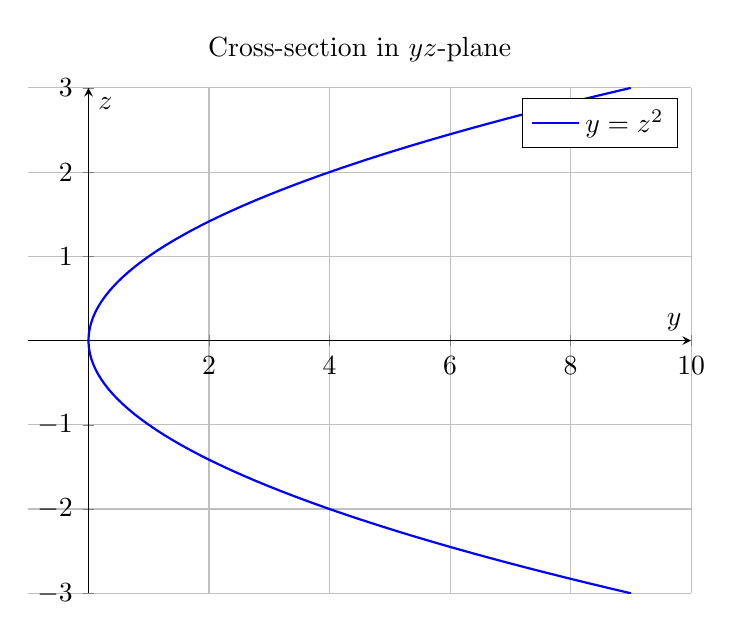
\begin{tikzpicture}
\begin{axis}[
    xlabel=$y$,
    ylabel=$z$,
    title={Cross-section in $yz$-plane},
    grid=major,
    width=10cm,
    height=8cm,
    axis lines=middle,
    xmin=-1, xmax=10,
    ymin=-3, ymax=3,
    legend style={at={(0.98,0.98)}, anchor=north east},
]
\addplot[blue, thick, domain=-3:3, samples=100] ({x^2}, {x});
\addlegendentry{$y = z^2$}
\end{axis}
\end{tikzpicture}
\end{document}
